\documentclass[a4paper,12pt]{article}
\usepackage[T1]{fontenc} % codifica dei font
\usepackage[utf8]{inputenc} % lettere accentate da tastiera
\usepackage[italian]{babel} % lingua del documento
\usepackage{url} % per scrivere gli indirizzi Internet
\usepackage{imakeidx}
\usepackage{amsmath}
\setlength\parindent{24pt}
\makeindex	
\usepackage{enumitem}
\usepackage{graphicx}
\graphicspath{ {./images/} }

\usepackage{float}

\usepackage{listings}
\lstset{breaklines=true}

\usepackage{listings}
\usepackage{xcolor}

\definecolor{codegreen}{rgb}{0,0.6,0}
\definecolor{codegray}{rgb}{0.5,0.5,0.5}
\definecolor{codepurple}{rgb}{0.58,0,0.82}
\definecolor{backcolour}{rgb}{0.95,0.95,0.92}

\lstdefinestyle{mystyle}{
    backgroundcolor=\color{backcolour},   
    commentstyle=\color{codegreen},
    keywordstyle=\color{magenta},
    numberstyle=\tiny\color{codegray},
    stringstyle=\color{codepurple},
    basicstyle=\ttfamily\footnotesize,
    breakatwhitespace=false,         
    breaklines=true,                 
    captionpos=b,                    
    keepspaces=true,                 
    numbers=left,                    
    numbersep=5pt,                  
    showspaces=false,                
    showstringspaces=false,
    showtabs=false,                  
    tabsize=2
}

\lstset{style=mystyle}



\begin{document}
\author{Daniel Xhakalliu}
\title{Calcolo Numerico Con Laboratorio Di MATLAB}
\maketitle
\clearpage
\tableofcontents
\clearpage



\section{Testi degli esercizi in MATLAB}
In seguito verranno enunciati gli esercizi dai quali abbiamo implementato dei programmi in MATLAB necessari per risolvere i problemi.
\subsection{Esercizio}
Scrivere un programma MATLAB che implementa l’algoritmo di valutazione del polinomio d'interpolazione in uno o più punti. Il programma deve:
\begin{itemize}
\item prendere in input tre vettori (a componenti reali) [$x_0, x_1,\dots, x_n$], [$y_0, y_1,\dots, y_n$], [$t_1,\dots, t_m$], con $x_0, x_1,\dots, x_n$ tutti distinti;
\item restituire in output il vettore [$p(t_1),\dots, p(t_m)$] che contiene le valutazioni nei punti $t_1,\dots, t_m$ del polinomio $p(x)$ interpolante i dati $(x_0, y_0),\dots, (x_n, y_n)$.
\end{itemize}
\subsection{Esercizio}
Scrivere un programma Matlab che implementa la formula dei trapezi. Il programma
deve:
\begin{itemize}
\item prendere in input gli estremi $a, b$ di un intervallo, una funzione $f(x)$ definita su $[a, b]$ e il numero $n\geq1$ di
sottointervalli in cui viene suddiviso $[a, b]$;
\item restituire in output $I_n$, l’approssimazione di
$\int_{a}^{b} f(x) \,dx$ data dalla formula dei trapezi di ordine $n$.
\end{itemize}

\subsection{Esercizio}
Usando i programmi creati per risolvere gli Esercizi 1.1 e 1.2, scrivere un programma
Matlab che implementa il metodo di estrapolazione. Il programma deve:
\begin{itemize}
\item prendere in input gli estremi $a, b$ di un intervallo, una funzione $f(x)$ definita su $[a, b]$ e un vettore
$[n_0, n_1, \dots, n_m]$ di numeri $n_0, n_1, \dots, n_m\geq1$ tutti distinti;
\item restituire in output il valore estrapolato $p(0)$, dove $p(x)$ è il polinomio d’interpolazione dei dati $(h_0^2, I_{n_{0}}), (h_1^2, I_{n_{1}}), \dots, (h_m^2, I_{n_{m}}) $ e $h_0, h_1,\dots, h_m$ sono i passi di discretizzazione delle formule dei trapezi $ I_{n_{0}}, I_{n_{1}}, \dots, I_{n_{m}}$ per approssimare
$\int_{a}^{b} f(x) \,dx$.
\end{itemize}


\section{Testi dei problemi in MATLAB}
\subsection{Problema}
Si consideri la funzione $\sqrt{x}$.
\begin{enumerate}[label=(\alph*)]
\item Sia $p(x)$ il polinomio d’interpolazione di $\sqrt{x}$ sui nodi
\begin{equation*}
x_0=0,  x_1=\frac{1}{64}, x_2=\frac{4}{64}, x_3=\frac{9}{64}, x_4=\frac{16}{64}, x_5=\frac{25}{64}, x_6=\frac{36}{64}, x_7=\frac{49}{64}, x_8=1.
\end{equation*}
Calcolare il vettore colonna 
\begin{equation*}
[p(\zeta_1)-\sqrt{\zeta_1}, p(\zeta_2)-\sqrt{\zeta_2},\dots, p(\zeta_{21})-\sqrt{\zeta_{21}}]^T
\end{equation*}
dove $\zeta_i = \frac{i-1}{20}$ per $i=1,\dots,21$ e osservare in che modo varia la differenza $p(\zeta_i)-\sqrt{\zeta_i}$ al variare di $i$
da 1 a 21.
\item Tracciare il grafico di $\sqrt{x}$ e di $p(x)$ sull’intervallo $[0, 1]$, ponendo i due grafici su un’unica figura e inserendo una legenda che ci dica qual è la funzione $\sqrt{x}$ e qual è il polinomio $p(x)$.
\end{enumerate}

\subsection{Problema}
Si consideri la funzione
\begin{equation*}
f(x)=e^x.
\end{equation*}
Per ogni intero $n\geq1$ indichiamo con $I_n$ la formula dei trapezi di ordine $n$ per approssimare
\begin{equation*}
I = \int_{0}^{1} f(x)\,dx = 1.7182818284590\dots
\end{equation*}
\begin{enumerate}[label=(\alph*)]
\item Per ogni fissato $\epsilon>0$ determinare un $n = n(\epsilon)$ tale che $|I-I_n|\leq\epsilon$.
\item Costruire una tabella che riporti vicino ad ogni $\epsilon\in\{10^{-1},10^{-2},\dots,10^{-10}\}$:
\begin{itemize}
\item il numero $n(\epsilon)$;
\item il valore $I_n$ per $n = n(\epsilon)$;
\item il valore esatto $I$ (in modo da confrontarlo con $I_n$);
\item l’errore $|I-I_n|$ (che deve essere $\leq\epsilon$).
\end{itemize}
\item Calcolare le approssimazioni di $I$ ottenute con le formule dei trapezi $I_2, I_4, I_8,I_{16}$ e confrontarle con
il valore esatto $I$.
\item Sia $p(x)$ il polinomio d’interpolazione dei valori $I_2, I_4, I_8,I_{16}$ sui nodi $h^2_2,h^2_4,h^2_8,h^2_{16},$ dove $h_2=\frac{1}{2}, h_4=\frac{1}{4},h_8=\frac{1}{8},h_{16}=\frac{1}{16}$ sono i passi di discretizzazione relativi alle formule dei trapezi $I_2, I_4, I_8,I_{16}$
rispettivamente. Calcolare $p(0)$ e confrontare $I_2, I_4, I_8,I_{16}, p(0)$ con il valore esatto $I$. Che cosa si
nota?
\end{enumerate}
\subsection{Problema}
Consideriamo la funzione $f(x) = x^2e^{-x}$ e indichiamo con $I_n$ la formula dei trapezi di ordine
$n$ per approssimare $I=\int_{0}^{1} f(x) \,dx $.
\begin{enumerate}[label=(\alph*)]
\item Calcolare $I$ prima manualmente e poi con la funzione simbolica \textbf{int} di MATLAB;
\item Calcolare $I_5, I_{10}, I_{20}, I_{40}$.
\item Calcolare $p(0)$, dove $p(x)$ è il polinomio d’interpolazione dei dati $(h^2_0, I_5),\\(h^2_1, I_{10}),(h^2_2, I_{20}),(h^2_3, I_{40}) $ e
$h_0, h_1, h_2, h_3$ sono i passi di discretizzazione delle formule dei trapezi $I_5, I_{10}, I_{20}, I_{40}$.
\item Riportare in una tabella:
\begin{itemize}
\item i valori $I_5, I_{10}, I_{20}, I_{40}, p(0)$;
\item gli errori $|I_{5}-I|,|I_{10}-I|,|I_{20}-I|,|I_{40}-I|,|p(0)-I|$ .
\end{itemize}
\item Posto $\epsilon=|p(0)-I|$, determinare un $n$ in modo tale che la formula dei trapezi $I_n$ fornisca un’approssimazione
di $I$ con errore $|I_n-I|\leq\epsilon$. Calcolare successivamente $I_n$ e verificare che effettivamente $|I_n-I|\leq\epsilon$.
\end{enumerate}


\section{Soluzioni ai problemi}
\subsection{Soluzione al problema 2.1}
\begin{enumerate}[label=(\alph*)]

\item Il vettore colonna è dato da:
\begin{equation*}
\begin{pmatrix}
                  0\\
   0.009373456935820\\
  -0.016624898598359\\
   0.006265159516694\\
   0.026059100541981\\
  -0.000000000000000\\
  -0.046798842893449\\
  -0.052843679514482\\
   0.019043791981465\\
   0.136657922266043\\
     0.195969221000565\\
   0.070222900207983\\
  -0.298665479678432\\
  -0.793827451939212\\
  -1.047857448417112\\
  -0.461689802877413\\
   1.600121563949947\\
   5.337600132745780\\
   9.648720381277604\\
  10.731478361986419\\
  -0.000000000000199\\
\end{pmatrix}
\end{equation*}
\item La figura seguente mostra il grafico di $\sqrt{x}$ e di $p(x)$ sull'intervallo $[0, 1]$:
\begin{center}
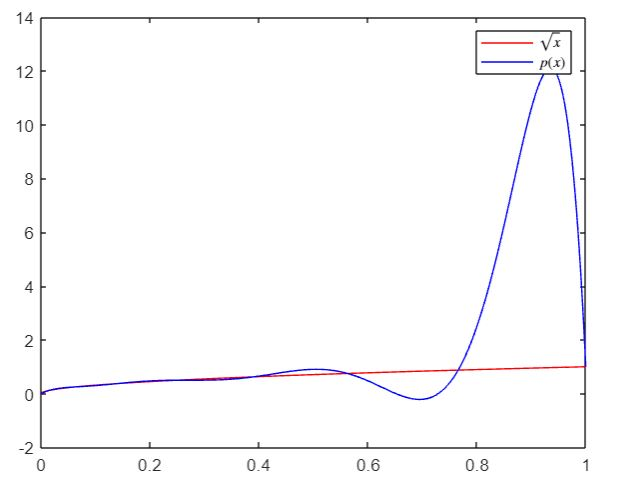
\includegraphics[width=8cm]{grafico}
\end{center}
\end{enumerate}

\subsection{Soluzione al problema 2.2}
\begin{enumerate}[label=(\alph*)]
\item Dato un qualsiasi $\epsilon>0$, la formula $n=\frac{0.4759448347}{\sqrt{\epsilon}
}$ determina un $n$ tale che $|I-I_n|\leq\epsilon$. 

\item  La tabella richiesta:
\begin{table}[h!]
  \begin{center}
    \label{tab:table1}
    \begin{tabular}{c|c|c|c|c} 
      $\epsilon$ & $n$ & $I_n$ & $I$ & $|I-I_n|$ \\
      \hline
       $10^{-1}$   &      2  &    1.75393109246483  &  1.71828182845905    & $3.56\cdot10^{-2}$\\
      $10^{-2}$   &      5 &    1.72400561978279   &  1.71828182845905     & $5.72\cdot10^{-3}$\\
     $10^{-3}$    &    16  &   1.71884112857999  &  1.71828182845905    & $5.59\cdot10^{-4}$\\
    $10^{-4}$     &   48  &  1.71834397651311  &  1.71828182845905    & $ 6.21\cdot10^{-5}$\\
     $10^{-5}$    &   151 &   1.71828810844886  &  1.71828182845905    & $6.27\cdot10^{-6}$\\
     $10^{-6}$    &   476  &  1.71828246043305  &  1.71828182845905    & $ 6.31\cdot10^{-7}$\\
     $10^{-7}$   &    1506   &    1.71828189159303   & 1.71828182845905    & $6.31\cdot10^{-8}$\\
     $10^{-8}$   &    4760  &   1.71828183477879   & 1.71828182845905    & $6.31\cdot10^{-9}$\\
     $10^{-9}$   &   15051 & 1.71828182909114   & 1.71828182845905    & $ 6.32\cdot10^{-10}$\\
     $10^{-10}$   &   47595   & 1.71828182852224  &  1.71828182845905    & $6.31\cdot10^{-11}$\\
     \end{tabular}
  \end{center}
\end{table}

\item In seguito vengono mostrate le approssimazioni di $I$ con le formule dei trapezi $I_2,I_4,I_8,I_{16}$ e gli errori commessi da essi.  
\begin{table}[h!]
  \begin{center}
    \begin{tabular}{c|c|c}
      $n$ & $I_n$ & $|I-I_n|$ \\
      \hline
       2 &   1.75393109246483    & $3.56\cdot10^{-2}$\\
     4  &  1.72722190455752  & $8.94\cdot10^{-3}$\\
     8  &  1.7205185921643  & $2.23\cdot10^{-3}$\\
    16  & 1.71884112857999 & $5.59\cdot10^{-4}$\\
    \end{tabular}
  \end{center}
\end{table}

\item Osservando la tabella successiva possiamo notare che al crescere di $n$ le approssimazioni usando la formula dei trapezi sono più accurate, ma il valore estrapolato $p(0)$ approssima commettendo l'errore più piccolo.

\begin{table}[H]
  \begin{center}
    \begin{tabular}{c|c|c|c}
      $n$ & $I_n$ & $I$ & $|I-I_n|$ \\
      \hline
       2 & 1.75393109246483  &  1.71828182845905     & $3.56\cdot10^{-2}$\\
    4 & 1.72722190455752 &   1.71828182845905  &   $8.94\cdot10^{-3}$\\
     8 & 1.7205185921643 &   1.71828182845905   &  $2.23\cdot10^{-3}$\\
    16 & 1.71884112857999  &  1.71828182845905  &  $5.59\cdot10^{-4}$\\
     & $p(0)$ & $I$ & $|I-p(0)|$\\
    \hline
      - & 1.71828182846039  &  1.71828182845905 &    $1.34\cdot10^{-12}$\\
    \end{tabular}
  \end{center}
\end{table}

\end{enumerate}
\subsection{Soluzione al problema 2.3}
\begin{enumerate}[label=(\alph*)]

\item Iniziamo calcolando manualmente l'integrale.
\begin{equation*}
\int_{0}^{1} x^2e^{-x}\,dx.
\end{equation*}
Integriamo per parti $e^{-x}x^2$,
\begin{equation*}
\int_{}^{} f \,dg=fg - \int_{}^{} g\,df
\end{equation*}
dove $f=x^2, dg=e^{-x}\,dx, df=2x\,dx, g=-e^{-x}: $
\begin{equation*}
\int_{0}^{1} x^2e^{-x}\,dx=(-e^{-x}x^2)\Big|_{0}^{1}+2\int_{0}^{1}e^{-x}x\,dx= -\frac{1}{e}+2\int_{0}^{1}e^{-x}x\,dx.
\end{equation*}
Integriamo per parti $e^{-x}x$,
\begin{equation*}
\int_{}^{} f \,dg=fg - \int_{}^{} g\,df
\end{equation*}
dove $f=x, dg=e^{-x}\,dx, df=\,dx, g=-e^{-x}: $
\begin{equation*}
-\frac{1}{e}+2\int_{0}^{1}e^{-x}x\,dx=-\frac{1}{e}+(-2e^{-x}x)\Big|_{0}^{1}+2\int_{0}^{1}e^{-x}\,dx=  -\frac{3}{e}+2\int_{0}^{1}e^{-x}\,dx.
\end{equation*}
Utilizzando il teorema fondamentale del calcolo integrale:
\begin{equation*}
-\frac{3}{e}+2\int_{0}^{1}e^{-x}\,dx=-\frac{3}{e}+(-2e^{-x})\Big|_{0}^{1}=2-\frac{5}{e}=0.160602794142788
\end{equation*}
Utilizzando la funzione \textbf{int} di MATLAB abbiamo che $I=2-\frac{5}{e}$, che è uguale alla nostra risposta.

\item Nella tabella seguente sono mostrati i valori di $I_5,I_{10},I_{20},I_{40}$:

\begin{table}[H]
  \begin{center}
    \begin{tabular}{c|c} 
      $n$ & $I_n$ \\
      \hline
    5 &   0.161816576820683\\
    10 &   0.160908578632096\\
    20  &  0.160679386811339\\
    40  &  0.160621951474857  \\   
         \end{tabular}
  \end{center}
\end{table}
\item  Sia $p(x)$ il polinomio d’interpolazione dei dati $(h^2_0, I_5),(h^2_1, I_{10}),(h^2_2, I_{20}),(h^2_3, I_{40}) $ dove
$h_0, h_1, h_2, h_3$ sono i passi di discretizzazione delle formule dei trapezi $I_5, I_{10}, I_{20}, I_{40}$. Il valore estrapolato $p(0)$ è uguale a 0.160602794142805.
\item La tabella richiesta: 
\begin{table}[H]
  \begin{center}
    \begin{tabular}{c|c|c}
      
     $n$ & $I_n$ & $|I_n-I|$ \\
      \hline
     5 & 0.161816576820683  &   $1.21\cdot10^{-3}$\\
    10 & 0.160908578632096  &  $3.05\cdot10^{-4}$\\
    20 & 0.160679386811339  &   $7.65\cdot10^{-5}$\\
    40 & 0.160621951474857  &  $1.91\cdot10^{-5}$\\
	   & $p(0)$ & $|p(0)-I|$\\
      \hline
    - &  0.160602794142805  &  $1.62\cdot10^{-14}$\\
      
    \end{tabular}
  \end{center}
\end{table}

\item Sia $\epsilon=|p(0)-I|=1.62\cdot10^{-14}$. Utilizzando la formula $n=\frac{0.4082482905}{\sqrt{\epsilon}}$, troviamo un $n=3209335$ tale che: 
\begin{equation*}
2.77\cdot10^{-17}=|I_n-I|\leq\epsilon=1.62\cdot10^{-14}
\end{equation*}
Calcolando $I_{3209335}$ otteniamo:
\begin{equation*}
I_{3209335} =  0.160602794142788
\end{equation*}
\end{enumerate}

\clearpage

\section{Appendice}
In questa sezione sono presenti tutti i programmi MATLAB utilizzati per svolgere gli esercizi e i problemi presenti in questo documento.
\subsection{Funzioni MATLAB}

\subsubsection{Metodo Ruffini Horner}
INPUT
\begin{description}
\item $x$: un vettore $[x_0,x_1, \dots, x_n]$ dove $x_0,x_1, \dots, x_n$ sono tutti distinti.
\item $y$: un vettore $[y_0,y_1, \dots, y_n]$.
\item $t$: un vettore $[t_0,t_1, \dots, t_m]$.
\end{description}
OUTPUT
\begin{description}
\item $PdiT$: il vettore $[p(t_0),p(t_1), \dots, p(t_m)]$ che contiene la valutazione nei punti $t_0, t_1,\dots,t_m$ del polinomio $p(x)$ interpolante i dati \\$(x_0,y_0),(x_1,y_1),\dots,(x_n,y_n)$.
\end{description}
\lstinputlisting[language=Matlab]{codes/RuffiniHorner.m}

\subsubsection{Formula dei Trapezi}
INPUT
\begin{description}
\item $a$: estremo inferiore dell'intervallo.
\item $b$: estremo superiore dell'intervallo.
\item $funx$: una funzione $f(x)$ definita su $[a, b]$.
\item $n$: il numero di sottointervalli in cui viene suddiviso $[a, b]$.
\end{description}
OUTPUT
\begin{description}
\item $I_n$: l'approssimazione $\int_{a}^{b}f(x)\,dx$ data dalla formula dei trapezi di ordine $n$.
\end{description}
\lstinputlisting[language=Matlab]{codes/FormulaDeiTrapezi.m}

\subsubsection{Valore estrapolato}
INPUT
\begin{description}
\item $a$: estremo inferiore dell'intervallo.
\item $b$: estremo superiore dell'intervallo.
\item $f$: una funzione $f(x)$ definita su $[a, b]$.
\item $n$: un vettore $[n_0, n_1, \dots, n_m]$ di numeri distinti.
\end{description}
OUTPUT
\begin{description}
\item $p0$: il valore estrapolato $p(0)$,dove $p(x)$ è il polinomio d’interpolazione dei dati $(h_0^2, I_{n_{0}}), (h_1^2, I_{n_{1}}), \dots, (h_m^2, I_{n_{m}}) $ e $h_0, h_1,\dots, h_m$ sono i passi di discretizzazione delle formule dei trapezi $ I_{n_{0}}, I_{n_{1}}, \dots, I_{n_{m}}$ per approssimare
$\int_{a}^{b} f(x) \,dx$.
\end{description}

\lstinputlisting[language=Matlab]{codes/Estrapolazione.m}



\subsection{Script MATLAB} 
\subsubsection{Script problema 2.1}
\begin{enumerate}[label=(\alph*)]
\item\phantom{-}\lstinputlisting[language=Matlab]{codes/es1/a.m}
\item\phantom{-}\lstinputlisting[language=Matlab]{codes/es1/b.m}
\end{enumerate}

\subsubsection{Script problema 2.2}
\begin{enumerate}[label=(\alph*)]
\item\phantom{-}\lstinputlisting[language=Matlab]{codes/es2/a.m}
\item\phantom{-}\lstinputlisting[language=Matlab]{codes/es2/b.m}
\item\phantom{-}\lstinputlisting[language=Matlab]{codes/es2/c.m}
\item\phantom{-}\lstinputlisting[language=Matlab]{codes/es2/d.m}
\end{enumerate}

\subsubsection{Script problema 2.3}
\begin{enumerate}[label=(\alph*)]
\item\phantom{-}\lstinputlisting[language=Matlab]{codes/es3/a.m}
\item\phantom{-}\lstinputlisting[language=Matlab]{codes/es3/b.m}
\item\phantom{-}\lstinputlisting[language=Matlab]{codes/es3/c.m}
\item\phantom{-}\lstinputlisting[language=Matlab]{codes/es3/d.m}
\item\phantom{-}\lstinputlisting[language=Matlab]{codes/es3/e.m}
\end{enumerate}

\end{document}